\documentclass[11pt,a4paper]{article}

% ====== PAQUETES ======
\usepackage[spanish]{babel}
\usepackage[T1]{fontenc}
\usepackage{libertinus}
\usepackage{tikz}
\usepackage{graphicx}
\usepackage{geometry}
\usepackage{tabularx}
\usepackage{xcolor}
\usepackage{fancyhdr}
\usepackage{titlesec}
\usepackage{chngcntr}
\usepackage{caption}
\usepackage{url}    
\usepackage{hyperref}
\usepackage{float}
\usepackage[cache=false]{minted}
\usepackage{pifont}
\usepackage{hyperref}
\newcommand{\cmark}{\ding{51}}

% ====== MÁRGENES ======
\geometry{top=2.5cm, bottom=3cm, left=2.5cm, right=2.5cm}
\setlength{\parindent}{0pt}

% ====== COLORES ======
\definecolor{azulceu}{RGB}{0,70,140}
\colorlet{azulceu}{azulceu!80!white}
\definecolor{grisclaro}{gray}{0.98}
\definecolor{codegray}{gray}{0.95}
\definecolor{linkblue}{RGB}{0, 102, 204}
\hypersetup{
    colorlinks=true,
    linkcolor=linkblue,
    urlcolor=linkblue,
    citecolor=linkblue
}

% ====== ENCABEZADO ======
\pagestyle{fancy}
\fancyhf{}
\fancyhead[L]{\small\textsc{Ingeniería Matemática\\Aprendizaje Automático}}
\fancyhead[R]{
\includegraphics[scale=0.13]{img/ceu.png}}
\fancyfoot[C]{\thepage}
\setlength{\headheight}{29.52pt}

% ====== TÍTULOS ======
\titleformat{\section}{\Large\bfseries\color{azulceu}}{\thesection}{1em}{}
\titleformat{\subsection}{\large\bfseries\color{grisclaro}}{\thesubsection}{1em}{}

% ====== INICIO DEL DOCUMENTO ======
\begin{document}
\begin{titlepage}
\begin{tikzpicture}[remember picture, overlay]

  % Fondo general gris claro
  \fill[grisclaro] (current page.south west) rectangle (current page.north east);

  % Franja vertical azul a la izquierda
  \fill[azulceu] (current page.south west) rectangle ([xshift=6cm]current page.north west);

  % Logo en la parte superior izquierda
  \node[anchor=north west, xshift=0cm, yshift=-1.2cm] at (current page.north west)
    {
\includegraphics[width=6cm]{img/ceubw.png}};

  % Título dentro de la franja azul
  \node[align=center, text=white, font=\bfseries\Huge] at ([xshift=3cm, yshift=-7cm]current page.north west)
    {MEMORIA\\PROYECTO};

  % Título principal elegante
  \node[align=center, text=azulceu, font=\bfseries\fontsize{20pt}{24pt}\selectfont] 
    at ([xshift=13.5cm, yshift=-15cm]current page.north west)
    {Aprendizaje Automático:\\[0.7em] \textsc{Predicción del Rendimiento Académico}};

  % Universidad
  \node[align=left, text=black, font=\bfseries\large] at ([xshift=13.5cm, yshift=10.5cm]current page.south west)
    {Universidad CEU San Pablo};

  % Autores del trabajo
  \node[align=center, text=black, font=\Large\itshape] at ([xshift=13.5cm, yshift=6.8cm]current page.south west)
    {David Ruiz Luque\\Alberto García Caballero\\Ricardo Marín Fernández-Conde};

  % Fecha centrada
  \node[align=center, text=black, font=\normalsize] at ([xshift=13.5cm, yshift=2.8cm]current page.south west)
    {15 de abril de 2025};

\end{tikzpicture}
\end{titlepage}


% ====== ÍNDICE ======
\newpage
\large
\tableofcontents
\thispagestyle{empty}
\newpage
\normalsize

% ====== REINICIAR NUMERACIÓN ======
\cleardoublepage
\pagenumbering{arabic}
\setcounter{page}{1}
\fancyfoot[C]{\raisebox{-10pt}{\thepage}}


% ====== RESUMEN ======

\begin{minipage}[t]{0.48\textwidth}
\raggedright
\textbf{Resumen}
\vspace{0.5em}

En esta práctica se ha desarrollado un sistema de extracción de información (web scraping) aplicado a documentos HTML, combinando herramientas modernas con modelos formales de la teoría de lenguajes. Para ello, se ha implementado un analizador léxico con PLY, basado en autómatas finitos deterministas (AFD), y se ha comparado su funcionamiento con la librería \texttt{BeautifulSoup}, ampliamente utilizada en entornos reales.

\vspace{0.5em}

El objetivo principal ha sido explorar hasta qué punto los conceptos formales —como lenguajes regulares, expresiones regulares y gramáticas— pueden emplearse para resolver problemas prácticos. Además de implementar ambos enfoques, se ha desarrollado un sistema de validación cruzada y una batería de pruebas sobre archivos HTML de distinta complejidad, lo que ha permitido evaluar la robustez y precisión del sistema.
\end{minipage}
\hfill
\begin{minipage}[t]{0.48\textwidth}
\raggedright
\textbf{Abstract}
\vspace{0.5em}

This project presents an information extraction (web scraping) system applied to HTML documents, combining formal language theory with practical tools. A lexical analyzer was implemented using PLY, based on deterministic finite automata (DFA), and compared to the \texttt{BeautifulSoup} library, widely used in real-world applications.

\vspace{0.5em}

The main objective was to explore the practical applicability of formal concepts —such as regular languages, regular expressions, and grammars— in solving real extraction tasks. Alongside the implementation of both methods, a cross-validation system and a set of tests over multiple HTML files were developed to evaluate robustness and accuracy.
\end{minipage}

\vspace{2.5em}

% ====== INTRODUCCIÓN ======
\section{Introducción}

El web scraping es una técnica ampliamente utilizada para extraer información automáticamente de páginas web. Aunque en la práctica suele abordarse desde herramientas de alto nivel como \texttt{BeautifulSoup}, en esta memoria se ha querido enfocar el problema desde una perspectiva diferente: aplicar conceptos teóricos de la asignatura de Teoría de la Computación, como los autómatas finitos deterministas (AFD), para resolver el mismo problema.

\medskip

La idea principal es construir autómatas que sean capaces de reconocer ciertas etiquetas HTML (concretamente \texttt{<a>} e \texttt{<img>}), y compararlos con un parser tradicional basado en el análisis del DOM. Esta aproximación permite comprobar de forma práctica hasta qué punto los modelos formales, vistos en un contexto teórico, pueden aplicarse a problemas del mundo real.

\medskip

El proyecto se ha desarrollado en Python, haciendo uso de herramientas como \texttt{PLY} para implementar un lexer con expresiones regulares, y \texttt{Graphviz} para generar los grafos de los autómatas. Además, se han utilizado páginas HTML de prueba y se ha incluido un sistema de comparación entre métodos.

\medskip

La práctica no solo ha servido para reforzar los conocimientos teóricos adquiridos en clase, sino también para experimentar con sus limitaciones y contrastarlos con enfoques modernos, valorando sus ventajas e inconvenientes.

%===== FUNDAMENTOS TEÓRICOS ======
\section{Fundamentos teóricos}

En esta sección se explican de forma sencilla los conceptos teóricos básicos que se han utilizado en la práctica. Nos centraremos en cómo los lenguajes regulares y los autómatas finitos deterministas (AFD) permiten detectar patrones en HTML, conectando así la teoría vista en clase con su aplicación práctica.

\subsection{Lenguajes formales y AFD}

Un \textbf{lenguaje formal} es un conjunto de cadenas sobre un alfabeto $\Sigma$. En esta práctica, las cadenas son fragmentos de código HTML y el alfabeto incluye caracteres como letras, números y símbolos especiales. Un lenguaje formal puede definirse mediante gramáticas o autómatas.

Entre los lenguajes formales, los más simples son los \textbf{lenguajes regulares}, los cuales pueden describirse mediante \textbf{expresiones regulares} y reconocerse utilizando autómatas finitos.

Un \textbf{autómata finito determinista} (AFD) es una 5-tupla:

\[
A = (Q, \Sigma, f, q_0, F)
\]

donde:
\begin{itemize}\setlength\itemsep{0.2em}
    \item $Q$ es el conjunto finito de estados.
    \item $\Sigma$ es el alfabeto de entrada.
    \item $f: Q \times \Sigma \rightarrow Q$ es la función de transición.
    \item $q_0 \in Q$ es el estado inicial.
    \item $F \subseteq Q$ es el conjunto de estados finales o de aceptación.
\end{itemize}

El autómata comienza en $q_0$ y avanza carácter a carácter según la función de transición $f$. Si al terminar la entrada está en un estado de $F$, la cadena se considera aceptada.

\subsection{Tokens y analizadores léxicos}

Un \textbf{token} es una unidad léxica que representa una estructura reconocible dentro del texto, como una palabra clave, un identificador o, en este caso, una etiqueta HTML.

Los analizadores léxicos (también llamados \textbf{lexers}) detectan estos tokens a partir de expresiones regulares. Cada expresión regular define un lenguaje regular, y por tanto puede ser representada por un AFD.

\medskip

En esta práctica, se ha utilizado la herramienta \texttt{PLY} (Python Lex-Yacc) para construir un lexer personalizado que actúe como un autómata, escaneando el texto HTML en busca de tokens específicos como \texttt{<a href="...">} o \texttt{<img src="...">}.

\subsection{Limitaciones del HTML como lenguaje}

Aunque el análisis sintáctico del HTML puede parecer sencillo a primera vista, en realidad HTML \textbf{no es un lenguaje regular}. Esto se debe a que permite estructuras anidadas, por ejemplo:

\begin{verbatim}
<div><a href="...">Texto <strong>enlace</strong></a></div>
\end{verbatim}

Reconocer correctamente este tipo de estructuras requiere una memoria adicional, como una pila, por lo que se necesita al menos un autómata a pila (AP).

Sin embargo, muchas tareas prácticas (como identificar etiquetas individuales bien formadas) pueden resolverse con expresiones regulares y AFDs. Por ello, esta práctica se centra en fragmentos simples de HTML, sin anidamiento.

%===== DISEÑO DEL PROYECTO ======
\section{Diseño del proyecto}

Para organizar el trabajo, el proyecto se ha dividido en varias partes. Por un lado, se ha implementado un \textit{lexer} con PLY, que actúa como un autómata para identificar patrones dentro del código HTML. Por otro lado, se ha desarrollado un parser con \texttt{BeautifulSoup}, una herramienta mucho más flexible y ampliamente utilizada en la actualidad. Finalmente, se ha añadido un sistema de comparación para analizar las diferencias entre ambos enfoques.

\subsection{Estructura del proyecto}

El proyecto se ha organizado en carpetas separadas para el código, los recursos de documentación y los archivos de salida:

\begin{itemize}
    \item \texttt{mi\_scraper/}: contiene todo el código Python, incluyendo el lexer, los autómatas, los scripts de test y el comparador.
    \item \texttt{mi\_scraper/html\_tests/}: incluye los archivos de prueba HTML sobre los que se realiza la extracción.
    \item \texttt{mi\_scraper/output/}: resultados de las extracciones realizadas tanto con BeautifulSoup como con PLY.
    \item \texttt{memoria/}: se encuentra la memoria en \LaTeX, junto con las imágenes generadas.
\end{itemize}

\subsection{Resumen de scripts principales}

\begin{table}[h]
\centering
\renewcommand{\arraystretch}{1.2}
\small
\begin{tabular}{|l|p{11cm}|}
\hline
\texttt{main.py} & Script principal que ejecuta el lexer y el parser, y genera los archivos de salida. \\ \hline
\texttt{lexer.py} & Define el lexer con PLY para reconocer etiquetas HTML específicas. \\ \hline
\texttt{parser.py} & Implementa el parser con PLY, que utiliza el lexer para extraer etiquetas. \\ \hline
\texttt{dom\_parser.py} & Utiliza \texttt{BeautifulSoup} para extraer las mismas etiquetas. \\ \hline
\texttt{cross\_test.py} & Compara los resultados obtenidos por ambos métodos. \\ \hline
\texttt{tests/test\_cases.py} & Contiene funciones de prueba automatizadas sobre los HTML de ejemplo. \\ \hline
\end{tabular}
\normalsize 
\end{table}

%===== WEB SCRAPING CON PLY ======
\section{Web scraping con PLY (Lexer y Parser)}
\subsection{Explicación de PLY y su papel en la práctica}

Para abordar el análisis léxico y sintáctico de páginas HTML se ha utilizado \texttt{PLY} (Python Lex-Yacc), una herramienta que implementa las funciones clásicas de \texttt{lex} y \texttt{yacc} dentro del lenguaje Python. Esta librería permite construir de forma declarativa un \textit{lexer} que identifique tokens a partir de expresiones regulares, así como un \textit{parser} capaz de procesar reglas sintácticas y detectar errores de estructura.

\medskip

El lexer actúa como un autómata finito determinista (AFD) que recorre carácter a carácter el contenido de un archivo HTML, identificando fragmentos que coincidan con patrones definidos. Estos patrones se expresan mediante expresiones regulares que definen tokens.

\medskip

Por otro lado, el parser trabaja sobre los tokens generados por el lexer y aplica reglas gramaticales para comprobar la estructura global del documento, como el anidamiento correcto de etiquetas. Esto permite detectar errores como etiquetas no cerradas o mal anidadas, los cuales no pueden ser reconocidos por un simple AFD.

\medskip

El uso de PLY en esta práctica permite ilustrar de forma práctica los conceptos de la asignatura, mostrando cómo los modelos teóricos como los autómatas y las gramáticas se pueden aplicar a tareas reales como el análisis de documentos HTML.

\subsection{Diseño de los AFD}

Para la parte léxica del proyecto se diseñaron dos autómatas finitos deterministas (AFD) que tienen como objetivo reconocer de forma precisa las etiquetas HTML más relevantes para esta práctica: los enlaces (\texttt{<a href="...">}) y las imágenes (\texttt{<img src="...">}).

\medskip

Ambos autómatas se construyeron a partir de las expresiones regulares definidas en el lexer y se generaron gráficamente mediante la herramienta \texttt{Graphviz}. Estas representaciones permiten visualizar cómo el lexer transita entre estados según los caracteres de entrada y en qué condiciones acepta una cadena como válida.

\medskip

\textbf{AFD para etiquetas de enlace (\texttt{<a href="...">}):}

\begin{figure}[H]
    \centering
    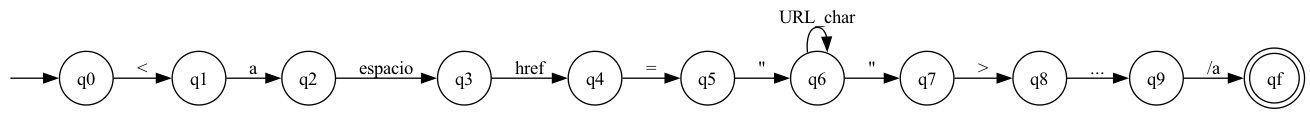
\includegraphics[width=0.9\textwidth]{img/afd_a_tag.png}
    \caption*{Autómata finito determinista para la etiqueta \texttt{<a href="...">}.}
\end{figure}

Este autómata comienza en un estado inicial que solo acepta el símbolo \texttt{<}. A partir de ahí, verifica carácter a carácter que la secuencia corresponda con la estructura típica de una etiqueta de enlace que contenga el atributo \texttt{href}. Si en cualquier punto se encuentra un carácter inesperado, el autómata no puede avanzar y rechaza la entrada.

\medskip

Cabe destacar que los estados trampa no han sido representados explícitamente en el gráfico ya que dificultan la visualización del mismo. Sin embargo, en la implementación real del lexer, estos estados son fundamentales para manejar entradas no válidas y evitar que el autómata continúe procesando cadenas incorrectas.

\vspace{1em}

\textbf{AFD para etiquetas de imagen (\texttt{<img src="...">}):}

\begin{figure}[H]
    \centering
    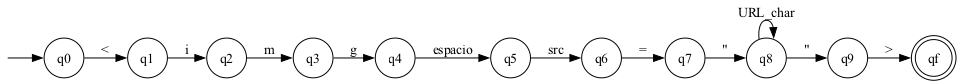
\includegraphics[width=0.9\textwidth]{img/afd_img_tag.png}
    \caption*{Autómata finito determinista para la etiqueta \texttt{<img src="...">}.}
\end{figure}

En este caso, el autómata valida que la cadena comience por \texttt{<img} y contenga el atributo \texttt{src}. A diferencia de la etiqueta \texttt{<a>}, no requiere una etiqueta de cierre, por lo que el autómata termina en un estado de aceptación tan pronto como se ha verificado la presencia del atributo y el cierre de la etiqueta.

\medskip

Estos autómatas muestran cómo los lenguajes regulares permiten capturar patrones bien definidos dentro del HTML. Sin embargo, como veremos más adelante, no son capaces de validar estructuras más complejas como el anidamiento correcto de etiquetas, lo cual justifica el uso posterior de un parser.

\subsection{Implementación del \texttt{lexer.py}}

El archivo \texttt{lexer.py} define el analizador léxico mediante la librería \texttt{PLY}. Este lexer está diseñado para escanear archivos HTML e identificar tokens específicos: principalmente etiquetas de enlace y de imagen.

\medskip

Cada token se define mediante una expresión regular asociada a una función. Cuando el texto de entrada coincide con la expresión, se genera un token correspondiente. Estos tokens son posteriormente utilizados tanto para la extracción directa como para el análisis sintáctico con el parser.

\medskip

A continuación se muestran las definiciones clave del lexer:

\begin{minted}[fontsize=\small, breaklines, bgcolor=codegray]{python}
# Token para enlaces con href
@lex.TOKEN(r'<a\s+href\s*=\s*"[^"]*"[^>]*>')
def t_A_TAG(t):
    return t
\end{minted}

Este patrón reconoce etiquetas \texttt{<a>} con atributo \texttt{href}, permitiendo cierto margen de espacios y otros atributos adicionales.

\begin{minted}[fontsize=\small, breaklines, bgcolor=codegray]{python}
# Token para imágenes con src
@lex.TOKEN(r'<img\s+src\s*=\s*"[^"]*"[^>]*>')
def t_IMG_TAG(t):
    return t
\end{minted}

De forma análoga, este token detecta etiquetas \texttt{<img>} que incluyan el atributo \texttt{src}. No se exige un cierre explícito de la etiqueta, ya que en HTML es común que estas aparezcan como self-closing.

\medskip

Además de estos tokens específicos, el lexer también define reglas para detectar etiquetas de apertura y cierre genéricas:

\begin{minted}[fontsize=\small, breaklines, bgcolor=codegray]{python}
# Etiquetas de apertura
@lex.TOKEN(r'<([a-zA-Z]+)(\s[^<>]*)?>')
def t_OPEN_TAG(t):
    t.value = t.value[1:].split()[0].lower()
    return t

# Etiquetas de cierre
@lex.TOKEN(r'</([a-zA-Z]+)\s*>')
def t_CLOSE_TAG(t):
    t.value = t.value[2:-1].strip().lower()
    return t
\end{minted}

Estas reglas permiten capturar otras etiquetas útiles para el análisis estructural, como \texttt{<body>}, \texttt{<p>}, \texttt{<div>}, etc. Su función principal es apoyar al parser en la detección de estructuras bien formadas o errores de balanceo.

\medskip

En conjunto, el archivo \texttt{lexer.py} actúa como un autómata que recorre el documento HTML y convierte su contenido en una secuencia de tokens, simplificando el análisis posterior.

\subsection{Implementación del \texttt{parser.py}}

El archivo \texttt{parser.py} define un analizador sintáctico utilizando la parte \texttt{yacc} de la librería \texttt{PLY}. Su propósito es validar la estructura general de un documento HTML, comprobando si las etiquetas están bien anidadas y correctamente balanceadas.

\medskip

Este parser opera sobre los tokens generados previamente por el lexer. Para ello, se definen una serie de reglas gramaticales recursivas que especifican cómo deben organizarse los elementos del HTML.

\medskip

A continuación se muestra un ejemplo simplificado de estas reglas:

\begin{minted}[fontsize=\small, breaklines, bgcolor=codegray]{python}
def p_document(p):
    'document : elements'
    pass

def p_elements(p):
    '''elements : element elements
                | element'''
    pass

def p_element(p):
    '''element : A_TAG
               | IMG_TAG
               | OPEN_TAG elements CLOSE_TAG'''
    if len(p) == 4 and p[1] != p[3]:
        print(f"Etiqueta no balanceada: <{p[1]}>...</{p[3]}>")
\end{minted}

La última regla es la más importante: permite validar que una etiqueta de apertura y su correspondiente etiqueta de cierre coincidan. Si no lo hacen, se imprime un mensaje de error indicando el desbalanceo detectado.

\medskip

Además, se incluye una función para capturar errores de sintaxis generales, como etiquetas mal formadas o fuera de lugar:

\begin{minted}[fontsize=\small, breaklines, bgcolor=codegray]{python}
def p_error(p):
    if p:
        print(f"Error de sintaxis en: {p.value}")
    else:
        print("Error de sintaxis al final del input")
\end{minted}

\medskip

El parser es compilado con la siguiente instrucción:

\begin{minted}[fontsize=\small, breaklines, bgcolor=codegray]{python}
parser = yacc.yacc()
\end{minted}

Esta llamada genera automáticamente los archivos \texttt{parsetab.py} y \texttt{parser.out}, que contienen las tablas de análisis y los estados del autómata construido internamente.

\medskip

Gracias a este componente, el sistema es capaz de detectar estructuras HTML incorrectas que no podrían ser identificadas por el lexer, como etiquetas abiertas que no se cierran o anidamientos incorrectos.

\subsection{Manejo de etiquetas mal formadas y estructura HTML}

Uno de los principales retos de esta práctica es que el lenguaje HTML, aunque simple en apariencia, permite estructuras anidadas y una gran variedad de formas sintácticas. Esto lo convierte en un lenguaje que no es regular, por lo que no puede ser reconocido completamente por un autómata finito determinista (AFD).

\medskip

El \textbf{lexer} basado en expresiones regulares funciona correctamente para detectar etiquetas bien formadas de tipo \texttt{<a href="...">} y \texttt{<img src="...">}. Sin embargo, no puede validar si estas etiquetas están correctamente anidadas ni si el documento HTML está balanceado estructuralmente. Esta limitación es esperada, ya que los AFD carecen de memoria para llevar seguimiento del contexto o del número de aperturas y cierres de etiquetas.

\medskip

Para resolver este problema, se desarrolló un \textbf{parser sintáctico} en \texttt{parser.py}, que permite analizar la estructura jerárquica del HTML mediante reglas recursivas. Gracias a este componente, es posible detectar errores comunes como:

\begin{itemize}
    \item Etiquetas abiertas que no se cierran correctamente.
    \item Anidamientos inválidos, como cerrar una etiqueta \texttt{<div>} con \texttt{</a>}.
    \item Cierre de etiquetas fuera de orden.
\end{itemize}

\medskip

Durante las pruebas, se comprobaron múltiples archivos HTML mal formados (ver Sección 7.4), y se observó que el parser era capaz de generar mensajes de error detallados para cada una de estas situaciones, mientras que el lexer las pasaba por alto si la etiqueta individual era sintácticamente válida.

\medskip

Esta combinación de lexer + parser permite simular un comportamiento similar al de un parser real de HTML, pero desde una perspectiva teórica basada en los conceptos vistos en la asignatura: \textbf{autómatas finitos} y \textbf{gramáticas independientes del contexto}.

%===== WEB SCRAPING CON BEAUTIFULSOUP ======
\section{Web scraping con BeautifulSoup (DOM)}
\subsection{Qué es BeautifulSoup y cómo se usa}

\texttt{BeautifulSoup} es una librería de Python ampliamente utilizada para realizar tareas de web scraping. A diferencia del enfoque basado en autómatas y expresiones regulares, esta herramienta trabaja a un nivel más alto, interpretando el documento HTML como una estructura jerárquica conocida como \textbf{DOM} (Document Object Model).

\medskip

Una vez cargado el documento, \texttt{BeautifulSoup} permite acceder a sus elementos mediante funciones como \texttt{find}, \texttt{find\_all} o búsquedas por atributos. Esto hace que sea extremadamente útil para extraer datos estructurados, incluso cuando el HTML está malformado o contiene errores.

\medskip

En el contexto de esta práctica, \textbf{BeautifulSoup se ha utilizado como método alternativo} al lexer+parser, con el objetivo de:

\begin{itemize}
    \item Extraer todas las etiquetas \texttt{<a>} que contengan un atributo \texttt{href}.
    \item Extraer todas las etiquetas \texttt{<img>} con atributo \texttt{src}.
    \item Contar la frecuencia de aparición de otras etiquetas relevantes del HTML.
\end{itemize}

\medskip

Este enfoque sirve como referencia para validar los resultados del lexer y del parser, y también permite comprobar qué ventajas ofrece una librería de propósito general frente a una solución construida desde los fundamentos teóricos de los lenguajes formales.

\subsection{Implementación del \texttt{dom\_parser.py}}

El archivo \texttt{dom\_parser.py} implementa el análisis del documento HTML utilizando la librería\\ \texttt{BeautifulSoup}. A diferencia del lexer basado en expresiones regulares, esta herramienta convierte automáticamente el código HTML en un árbol DOM, lo que facilita enormemente la navegación por sus elementos.

\medskip

La implementación comienza cargando el contenido del archivo HTML y creando un objeto\\ \texttt{BeautifulSoup} que representa su estructura:

\begin{minted}[fontsize=\small, breaklines, bgcolor=codegray]{python}
with open(html_file, encoding='utf-8') as f:
    html = f.read()

soup = BeautifulSoup(html, 'html.parser')
\end{minted}

\medskip

Una vez cargado, se realiza la extracción de enlaces e imágenes de forma muy directa, filtrando aquellas etiquetas que contengan los atributos deseados:

\begin{minted}[fontsize=\small, breaklines, bgcolor=codegray]{python}
# Extraer enlaces
links = [a['href'] for a in soup.find_all('a', href=True)]

# Extraer imágenes
images = [img['src'] for img in soup.find_all('img', src=True)]
\end{minted}

\medskip

Además de la extracción básica, el script cuenta el número de apariciones de otras etiquetas comunes como \texttt{<div>}, \texttt{<p>}, \texttt{<span>}, \texttt{<table>}, entre otras, y muestra un resumen por consola:

\begin{minted}[fontsize=\small, breaklines, bgcolor=codegray]{python}
tag_stats = {tag: len(soup.find_all(tag)) for tag in tags_to_check}

for tag, count in tag_stats.items():
    print(f"{tag}: {count}")
\end{minted}

\medskip

Finalmente, los enlaces e imágenes extraídos se guardan en archivos de texto dentro de la carpeta \texttt{output/}, lo que permite comparar los resultados con los obtenidos mediante PLY:

\begin{minted}[fontsize=\small, breaklines, bgcolor=codegray]{python}
Path("output/links_bs.txt").write_text("\\n".join(links))
Path("output/images_bs.txt").write_text("\\n".join(images))
\end{minted}

\medskip

Este enfoque destaca por su sencillez y robustez, ya que \texttt{BeautifulSoup} es capaz de tolerar errores de sintaxis en el HTML y continuar el análisis sin interrupciones. Esto contrasta con el comportamiento más estricto del parser implementado con PLY.

\subsection{Extracción de etiquetas y estadísticas}

Además de identificar enlaces e imágenes, el script \texttt{dom\_parser.py} genera un pequeño análisis estadístico del documento HTML. Esto se realiza contando la cantidad de veces que aparecen determinadas etiquetas de interés en el archivo de entrada.

\medskip

Las etiquetas analizadas incluyen tanto las relevantes para la extracción de contenido (\texttt{<a>}, \texttt{<img>}) como otras etiquetas HTML comunes:

\begin{minted}[fontsize=\small, breaklines, bgcolor=codegray]{python}
tags_to_check = ["a", "img", "br", "div", "li", "ul", 
                 "p", "span", "table", "td", "tr"]
\end{minted}

Se construye un diccionario que asocia cada etiqueta con el número de apariciones encontradas por \texttt{BeautifulSoup}:

\begin{minted}[fontsize=\small, breaklines, bgcolor=codegray]{python}
tag_stats = {tag: len(soup.find_all(tag)) for tag in tags_to_check}
\end{minted}

Posteriormente, el script imprime los resultados en consola, lo que permite tener una visión general del contenido HTML:

\begin{minted}[fontsize=\small, breaklines, bgcolor=codegray]{python}
print("\\n Estadísticas de etiquetas HTML:")
for tag, count in tag_stats.items():
    print(f"{tag}: {count}")
\end{minted}

\medskip

Este análisis es útil para validar los archivos de prueba utilizados y observar cómo varían según el caso. También ayuda a justificar las diferencias observadas en el comportamiento de los analizadores PLY y BS4, especialmente cuando se trabaja con HTML mal formado o documentos de estructura compleja.

\medskip

En resumen, la inclusión de estadísticas no solo permite comprobar que el análisis se realiza correctamente, sino que también facilita la interpretación de los resultados en la comparativa entre métodos.

\subsection{Ventajas y flexibilidad frente a PLY}

El enfoque basado en \texttt{BeautifulSoup} presenta una serie de ventajas prácticas frente al análisis con PLY, especialmente cuando se trabaja con archivos HTML reales, que frecuentemente contienen errores de sintaxis, etiquetas mal cerradas o estructuras anidadas complejas.

\medskip

A diferencia del lexer y parser implementados con PLY, que requieren que el HTML tenga una estructura bien definida para poder ser analizado correctamente, \texttt{BeautifulSoup} incluye mecanismos internos de corrección y recuperación de errores. Esto le permite analizar documentos imperfectos sin generar interrupciones ni fallos de ejecución.

\medskip

Algunas de las principales ventajas observadas son:

\begin{itemize}
    \item \textbf{Tolerancia a errores}: es capaz de interpretar HTML mal formado, insertando automáticamente etiquetas faltantes o corrigiendo jerarquías inválidas.
    \item \textbf{Simplicidad de uso}: permite acceder directamente a las etiquetas mediante métodos como\\ \texttt{find\_all}, sin necesidad de definir expresiones regulares ni reglas gramaticales.
    \item \textbf{Versatilidad}: soporta búsquedas por nombre de etiqueta, atributos, clases CSS, texto contenido y más.
\end{itemize}

\medskip

No obstante, estas ventajas vienen con una contrapartida: al abstraer los detalles del proceso de análisis, \texttt{BeautifulSoup} oculta el funcionamiento interno y no permite observar directamente cómo se realiza el reconocimiento de patrones, lo que puede dificultar su uso con fines educativos o de validación formal.

\medskip

Por el contrario, el enfoque con PLY, aunque más estricto y sensible a errores, permite comprender en profundidad cómo funcionan los analizadores léxicos y sintácticos, mostrando de forma explícita los errores encontrados y ofreciendo una experiencia más cercana a los conceptos teóricos vistos en la asignatura.

\medskip

Por tanto, ambos enfoques son complementarios: mientras que PLY proporciona una base sólida para comprender el funcionamiento interno del análisis de lenguajes, \texttt{BeautifulSoup} ofrece una solución eficaz para trabajar con documentos HTML en entornos reales.

%===== COMPARATIVA ENTRE MÉTODOS ======
\section{CrossTest: Comparación de resultados}
\subsection{Explicación de \texttt{cross\_test.py}}

Para validar la consistencia entre los resultados obtenidos con PLY y los obtenidos con \texttt{BeautifulSoup}, se ha implementado un script llamado \texttt{cross\_test.py}. Este componente compara los archivos de salida generados por ambos métodos, tanto para enlaces como para imágenes.

\medskip

La lógica del script es sencilla: abre los archivos \texttt{links\_ply.txt}, \texttt{links\_bs.txt}, \texttt{images\_ply.txt} e \texttt{images\_bs.txt}, y compara sus contenidos. Si ambas listas coinciden exactamente (sin importar el orden), se considera que el análisis ha sido consistente.

\medskip

A continuación se muestra un fragmento relevante del código:

\begin{minted}[fontsize=\small, breaklines, bgcolor=codegray]{python}
def comparar_resultados(archivo1, archivo2):
    conjunto1 = set(Path(archivo1).read_text().splitlines())
    conjunto2 = set(Path(archivo2).read_text().splitlines())
    return conjunto1 == conjunto2
\end{minted}

\medskip

Posteriormente, se llama a esta función para comparar los enlaces y las imágenes extraídos por ambos métodos:

\begin{minted}[fontsize=\small, breaklines, bgcolor=codegray]{python}
links_ok = comparar_resultados("output/links_ply.txt", "output/links_bs.txt")
imgs_ok = comparar_resultados("output/images_ply.txt", "output/images_bs.txt")
\end{minted}

En función del resultado, el script muestra un mensaje indicando si hay coincidencia o no:

\begin{minted}[fontsize=\small, breaklines, bgcolor=codegray]{python}
if links_ok:
    print("Enlaces coinciden")
else:
    print("DIFERENCIA en enlaces")
\end{minted}

\medskip

Este comparador resulta especialmente útil para evaluar la fiabilidad del lexer y parser implementados con PLY. Si ambos métodos coinciden en todos los casos, se puede concluir que el reconocimiento realizado por los autómatas es correcto, al menos en lo que respecta a las etiquetas objetivo de esta práctica.

\subsection{Validación cruzada entre PLY y BS4}

Tras la implementación de ambos analizadores y el desarrollo del script de comparación, se procedió a validar su comportamiento mediante múltiples archivos de prueba. En todos los casos se analizó la extracción de enlaces e imágenes, contrastando los resultados obtenidos por PLY (lexer + parser) y por \texttt{BeautifulSoup}.

\medskip

La validación cruzada reveló un comportamiento muy positivo: en todos los archivos de prueba, los resultados fueron coincidentes. Esto sugiere que, a pesar de sus limitaciones estructurales, el lexer y parser diseñados con PLY fueron capaces de identificar correctamente las etiquetas HTML objetivo y extraer la misma información que un analizador de propósito general como \texttt{BeautifulSoup}.

\medskip

Además, se observó que incluso en documentos HTML mal formados (con etiquetas sin cerrar, estructuras desordenadas o jerarquías incorrectas) ambos métodos lograron recuperar la misma información. Esto refuerza la idea de que el reconocimiento de patrones individuales, como las etiquetas \texttt{<a href="...">} o \texttt{<img src="...">}, puede abordarse con éxito utilizando técnicas formales basadas en autómatas finitos.

\medskip

No obstante, también se evidenció que el parser implementado con PLY resulta más estricto y menos tolerante a errores, ya que emite advertencias cuando las etiquetas están mal balanceadas. En cambio, \texttt{BeautifulSoup} ignora esos problemas y continúa el análisis normalmente, lo cual puede ser útil en entornos productivos pero menos formativo desde un punto de vista académico.

\medskip

En definitiva, esta validación cruzada permite confiar en la efectividad del sistema desarrollado y demuestra que los modelos teóricos aplicados en este proyecto tienen un alcance práctico significativo.

\subsection{Comentarios sobre resultados consistentes}

El análisis de los archivos de prueba reveló una alta consistencia entre los resultados obtenidos por los dos métodos implementados: el lexer y parser construidos con PLY, y el analizador de DOM basado en \texttt{BeautifulSoup}. A continuación se destacan algunas observaciones relevantes que permiten interpretar mejor estos resultados:

\begin{itemize}
    \item En todos los casos, tanto PLY como BeautifulSoup identificaron el mismo número de enlaces e imágenes, incluso en documentos mal estructurados. Esto refuerza la fiabilidad del enfoque basado en autómatas para reconocer patrones léxicos específicos.

    \item En archivos como \texttt{prueba3.html} y \texttt{prueba6.html}, que presentan etiquetas mal cerradas, anidamientos incorrectos o errores de sintaxis, el parser detectó múltiples errores, pero aún así se logró extraer correctamente la información deseada.

    \item El sistema de comparación no sólo valida la coincidencia de los datos, sino que también actúa como una verificación cruzada: si un método produce un resultado diferente, el error puede detectarse rápidamente revisando ambos archivos de salida.

    \item En el caso del lexer con PLY, el número de enlaces e imágenes coincide siempre que las etiquetas estén correctamente formadas en su versión básica. En cambio, BeautifulSoup puede extraer información útil incluso de etiquetas incompletas, lo cual puede considerarse tanto una ventaja como una fuente potencial de ruido.

    \item La ejecución repetida del script \texttt{run\_all.sh} sobre cada archivo de prueba mostró que el comportamiento era estable, consistente y predecible, lo que demuestra que el sistema es robusto ante entradas diversas.
\end{itemize}

Estas observaciones confirman que el diseño del sistema ha sido eficaz a la hora de combinar la precisión del análisis léxico con la flexibilidad del análisis estructural, ofreciendo una herramienta sólida para tareas de extracción de información en HTML.

\subsection{Tabla de cobertura de pruebas (PLY vs BS4)}

A continuación se muestra la tabla revisada que resume el comportamiento de ambos métodos para distintos archivos HTML:

\begin{table}[H]
\renewcommand{\arraystretch}{1.3}
\small
\begin{tabularx}{\textwidth}{|l|c|c|>{\raggedright\arraybackslash}X|c|c|c|c|}
\hline
\textbf{Archivo} & \textbf{Enl. PLY} & \textbf{Img. PLY} & \textbf{Balanceo HTML (parser)} & \textbf{Enl. BS4} & \textbf{Img. BS4} & \textbf{Links} & \textbf{Imgs} \\
\hline
\texttt{prueba1.html} & 0 & 0 & Error de sintaxis (falta apertura) & 0 & 0 & \cmark & \cmark \\
\texttt{prueba2.html} & 1 & 1 & \texttt{<br>} mal cerrado dentro de \texttt{<a>} & 1 & 1 & \cmark & \cmark \\
\texttt{prueba3.html} & 2 & 1 & Varias etiquetas no balanceadas (\texttt{<area>}) & 2 & 1 & \cmark & \cmark \\
\texttt{prueba4.html} & 1 & 1 & \texttt{<p>} y \texttt{<body>} sin cierre correcto & 1 & 1 & \cmark & \cmark \\
\texttt{prueba5.html} & 1 & 1 & \texttt{<a>} mal anidado dentro de \texttt{<p>} & 1 & 1 & \cmark & \cmark \\
\texttt{prueba6.html} & 48 & 14 & Múltiples errores de anidamiento y sintaxis & 48 & 14 & \cmark & \cmark \\
\hline
\end{tabularx}
\caption*{Resultados de la comparación entre PLY y BeautifulSoup.}
\end{table}

\medskip

Como puede observarse, todos los archivos presentan problemas de estructura HTML que son detectados por el parser con PLY. Sin embargo, tanto el lexer como el analizador con \texttt{BeautifulSoup} son capaces de extraer correctamente los enlaces e imágenes previstos. Las comprobaciones cruzadas confirman la coincidencia de resultados, validando la consistencia entre ambos enfoques.

%===== PRUEBAS DE EJECUCIÓN Y RESULTADOS ======
\section{Pruebas de ejecución y resultados}

En esta sección se muestran los resultados prácticos obtenidos al ejecutar el sistema completo sobre distintos archivos HTML de prueba. Para facilitar la ejecución, se desarrolló un script llamado \texttt{run\_all.sh} que automatiza el análisis completo con PLY, BeautifulSoup y la comparación cruzada.

\subsection{Ejecución del sistema completo}

A continuación se muestra un ejemplo de ejecución del script sobre el archivo \texttt{prueba3.html}, el cual contiene varias etiquetas mal balanceadas:

\begin{figure}[H]
    \centering
    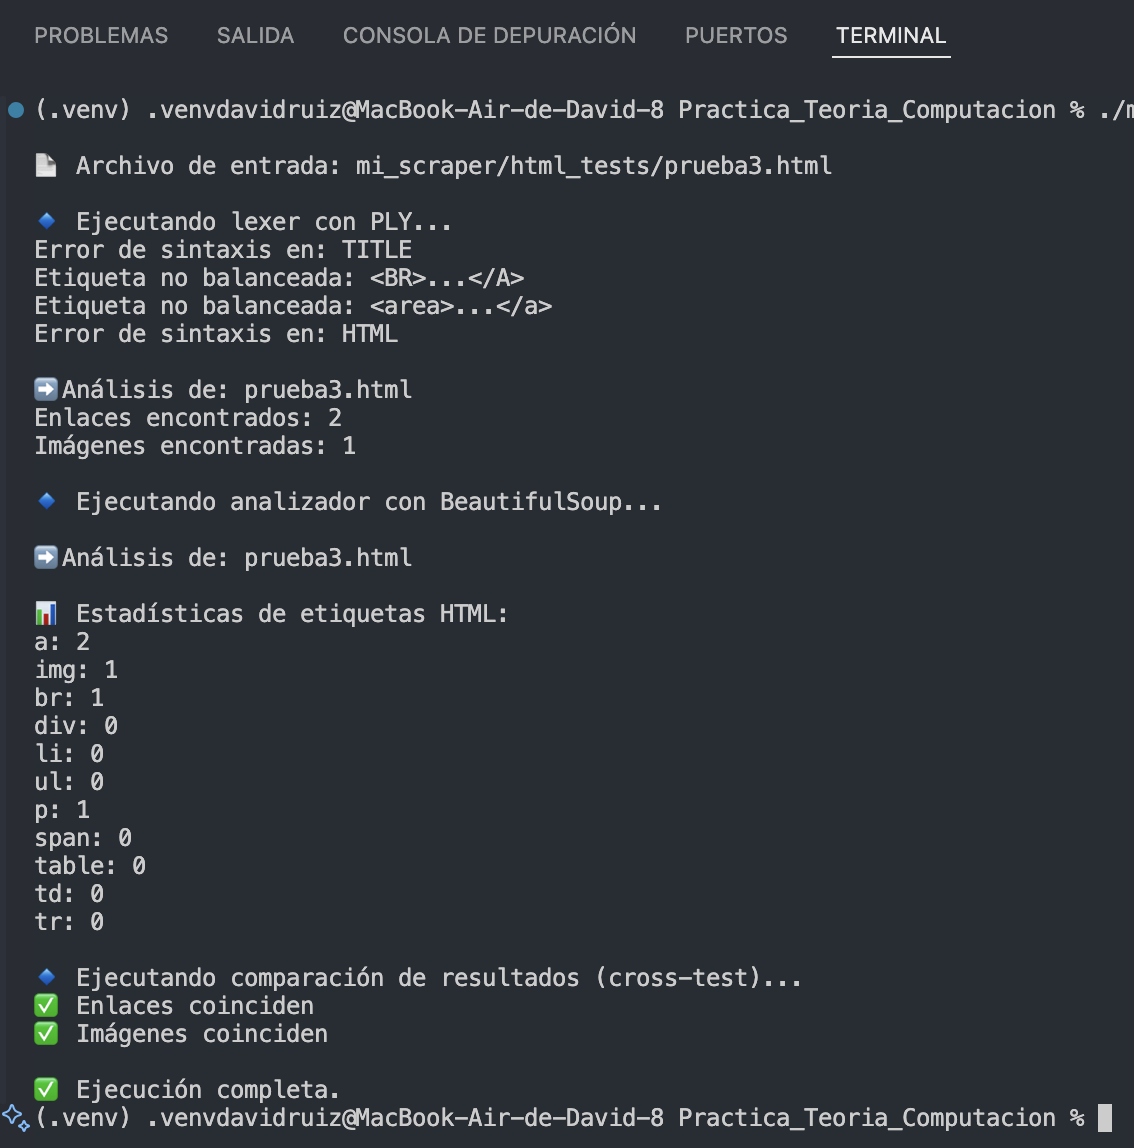
\includegraphics[width=0.6\textwidth]{img/ejecucion_prueba3.png}
    \caption*{Ejecución del script \texttt{run\_all.sh} sobre \texttt{prueba3.html}.}
\end{figure}

Como puede observarse, el parser detecta varios errores de sintaxis y etiquetas mal cerradas. A pesar de ello, tanto el lexer como BeautifulSoup logran extraer correctamente los enlaces e imágenes del documento.

\subsection{Archivos de salida generados}

El sistema crea automáticamente archivos de texto en la carpeta \texttt{output/}, donde se almacenan los resultados de la extracción realizada por ambos métodos. Por ejemplo:

\begin{itemize}
    \item \texttt{output/links\_ply.txt} — enlaces encontrados con el lexer.
    \item \texttt{output/images\_bs.txt} — imágenes encontradas con BeautifulSoup.
\end{itemize}

A continuación se muestra el contenido de uno de estos archivos para el caso de prueba anterior:

\begin{minted}[fontsize=\small, breaklines, bgcolor=codegray]{text}
http://www.bbc.co.uk
http://www.ibm.com
\end{minted}

Estos resultados confirman que la extracción es funcional incluso cuando el documento HTML contiene errores estructurales.

\subsection{Comprobación cruzada de resultados}

Como se ha explicado en la sección anterior, el script \texttt{cross\_test.py} compara los archivos de salida y verifica si ambos métodos producen resultados coincidentes.

\begin{figure}[H]
    \centering
    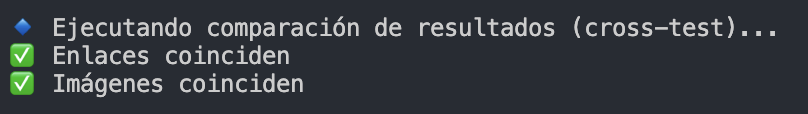
\includegraphics[width=0.6\textwidth]{img/cross_test_ok.png}
    \caption*{Verificación cruzada de resultados con \texttt{cross\_test.py}.}
\end{figure}

En todos los casos de prueba, se observó una coincidencia perfecta entre los enlaces e imágenes extraídos por PLY y los obtenidos por \texttt{BeautifulSoup}. Esto valida la efectividad del enfoque basado en autómatas finitos y gramáticas simplificadas para tareas prácticas de web scraping.

\subsection{Detección de errores sintácticos}

Uno de los aspectos más relevantes del parser implementado con PLY es su capacidad para identificar errores estructurales en el HTML, como etiquetas mal cerradas, anidamientos incorrectos o cierres fuera de lugar. A continuación se muestra un ejemplo real:

\begin{figure}[H]
    \centering
    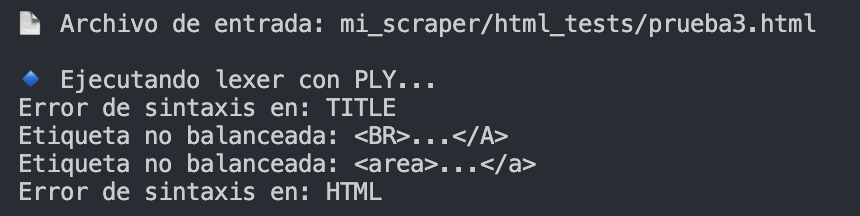
\includegraphics[width=0.6\textwidth]{img/errores_parser.png}
    \caption*{Mensajes de error generados por el parser ante etiquetas no balanceadas.}
\end{figure}

Estos mensajes son útiles tanto para validar la calidad del documento HTML como para ilustrar cómo un analizador sintáctico puede utilizar reglas formales para detectar errores.

\subsection{Tests unitarios}

Para validar el funcionamiento interno del lexer y del sistema de análisis desarrollado, se implementó un archivo de pruebas automáticas en \texttt{Python} utilizando la librería estándar \texttt{unittest}. Estas pruebas están definidas en el archivo:

\begin{minted}[fontsize=\small, breaklines, bgcolor=codegray]{text}
mi_scraper/tests/test_cases.py
\end{minted}

\medskip

El objetivo principal de los tests es asegurar que:

\begin{itemize}
    \item Las etiquetas \texttt{<a href="...">} y \texttt{<img src="...">} se reconocen correctamente como tokens por parte del lexer.
    \item La función principal \texttt{analyze\_html} extrae correctamente enlaces e imágenes desde un documento HTML.
    \item No se detectan enlaces inexistentes en documentos vacíos o sin etiquetas \texttt{<a>}.
\end{itemize}

A continuación se muestra un extracto relevante del archivo de pruebas, con ejemplos de validación de tokens:

\begin{minted}[fontsize=\small, breaklines, bgcolor=codegray]{python}
def test_detect_single_a_tag(self):
    html = '<a href="https://example.com">Link</a>'
    lexer.input(html)
    tokens = [tok for tok in lexer if tok.type == 'A_TAG']
    self.assertEqual(len(tokens), 1)
    self.assertEqual(tokens[0].value, 'https://example.com')
\end{minted}

Esta prueba asegura que se detecta correctamente un único enlace en el documento, y que el valor del token corresponde exactamente con la URL contenida en el atributo \texttt{href}.

\medskip

Además, se incluye una prueba para la extracción conjunta de enlaces e imágenes usando la función principal del sistema:

\begin{minted}[fontsize=\small, breaklines, bgcolor=codegray]{python}
def test_extract_links_and_images(self):
    html = '''
    <a href="http://link.com">Test</a>
    <img src="image.jpg">
    '''
    with tempfile.NamedTemporaryFile(mode="w+", suffix=".html") as f:
        f.write(html)
        f.flush()
        links, images = analyze_html(f.name)

    self.assertEqual(links[0], 'http://link.com')
    self.assertEqual(images[0], 'image.jpg')
\end{minted}

\medskip

Esta prueba permite comprobar que el flujo completo de análisis (lexer + parser) se ejecuta correctamente sobre un documento HTML creado de forma temporal, sin necesidad de guardar archivos permanentes.

\medskip

\textbf{Resultado de ejecución:} Todos los tests pasaron satisfactoriamente, lo que demuestra que el sistema de extracción está funcionando como se espera:

\begin{minted}[fontsize=\small, breaklines, bgcolor=codegray]{text}
....
----------------------------------------------------------------------
Ran 4 tests in 0.004s

OK
\end{minted}

\medskip

Este sistema de pruebas contribuye a mantener la fiabilidad del proyecto y garantiza que las funciones clave se comportan correctamente, incluso si en el futuro se realizan modificaciones o mejoras en el código base.


%===== CONCLUSIONES ======
\section{Conclusiones}

Este proyecto ha servido para poner en práctica conceptos de autómatas y gramáticas aplicados al análisis de HTML. Se ha comprobado que, aunque las herramientas teóricas como PLY funcionan bien para tareas concretas, soluciones como BeautifulSoup son más flexibles y robustas para HTML real. La comparación y las pruebas han mostrado que ambos métodos pueden ser fiables para extraer información sencilla.

\medskip

Sin embargo, el enfoque basado en autómatas y gramáticas permite comprender en profundidad los límites de los lenguajes regulares y el papel de los analizadores léxicos y sintácticos. Se ha evidenciado que, aunque los AFD son útiles para reconocer patrones simples, no pueden validar la estructura completa de HTML debido a su naturaleza no regular. El uso de un parser con reglas recursivas ha permitido detectar errores de anidamiento y balanceo, reforzando la importancia de las gramáticas independientes del contexto en el análisis de lenguajes más complejos.

\medskip

Por otro lado, BeautifulSoup ha demostrado ser una herramienta muy eficaz y tolerante a errores, lo que la hace idónea para aplicaciones prácticas de scraping en entornos reales. Su facilidad de uso y capacidad para manejar HTML mal formado justifican su popularidad en la industria.

\medskip

En resumen, la experiencia ha sido útil para entender mejor cómo se conectan la teoría y la práctica en el análisis de lenguajes. El trabajo realizado ha permitido valorar tanto la potencia de los modelos formales como la necesidad de herramientas prácticas en el desarrollo de soluciones reales, y ha reforzado la importancia de una formación sólida en los fundamentos teóricos de la asignatura.

\vspace{1em}

%===== BIBLIOGRAFÍA ======
\newpage
\addcontentsline{toc}{section}{Bibliografía}
\begin{thebibliography}{9}

\bibitem{Aho2007}
Aho, A. V., Lam, M. S., Sethi, R., \& Ullman, J. D. (2007).  
\textit{Compiladores: Principios, técnicas y herramientas}.  
Pearson Educación. Obra clásica sobre teoría de compiladores, autómatas, gramáticas y análisis léxico-sintáctico.

\bibitem{BeazleyPLY}
Beazley, D. (2023).  
\textit{PLY (Python Lex-Yacc) Documentation}.  
Disponible en: \url{https://www.dabeaz.com/ply/}  
Documentación oficial de la librería utilizada para construir analizadores léxicos y sintácticos en Python.

\bibitem{BeautifulSoup}
Richardson, L. (2023).  
\textit{BeautifulSoup Documentation}.  
Disponible en: \url{https://www.crummy.com/software/BeautifulSoup/}  
Manual y referencias para el uso del parser HTML más extendido en Python.

\bibitem{HTMLSpec}
WHATWG. (2024).  
\textit{HTML Living Standard}.  
Disponible en: \url{https://html.spec.whatwg.org/}  
Especificación oficial y actualizada del lenguaje HTML mantenida por el grupo WHATWG.

\bibitem{Graphviz}
Graphviz Team. (2024).
Disponible en: \url{https://graphviz.org/}  
Herramienta empleada para la generación visual de los autómatas finitos representados en esta práctica.

\bibitem{PythonDocs}
Python Software Foundation. (2024).  
\textit{Documentación oficial de Python}.  
Disponible en: \url{https://docs.python.org/3/}  
Referencia completa del lenguaje de programación utilizado en el desarrollo del proyecto.

\end{thebibliography}


\end{document}



\end{document}